% Editable TikZ version of methodology_flowchart.pdf (same content). Compile on Overleaf with pdfLaTeX.
% Standalone document; to embed inside the paper instead, copy the tikzpicture environment and
% add \usepackage{tikz} \usetikzlibrary{positioning,arrows.meta,calc} to the preamble.
\documentclass[border=4pt]{standalone}
\usepackage[T1]{fontenc}
\usepackage{amsmath}
\usepackage{tikz}
\usetikzlibrary{positioning,arrows.meta,calc}
\definecolor{cBlue}{HTML}{2A78D6}
\definecolor{cOrange}{HTML}{EB6834}
\definecolor{cAqua}{HTML}{1BAF7A}
\definecolor{cGrey}{HTML}{6B6B6B}
\begin{document}
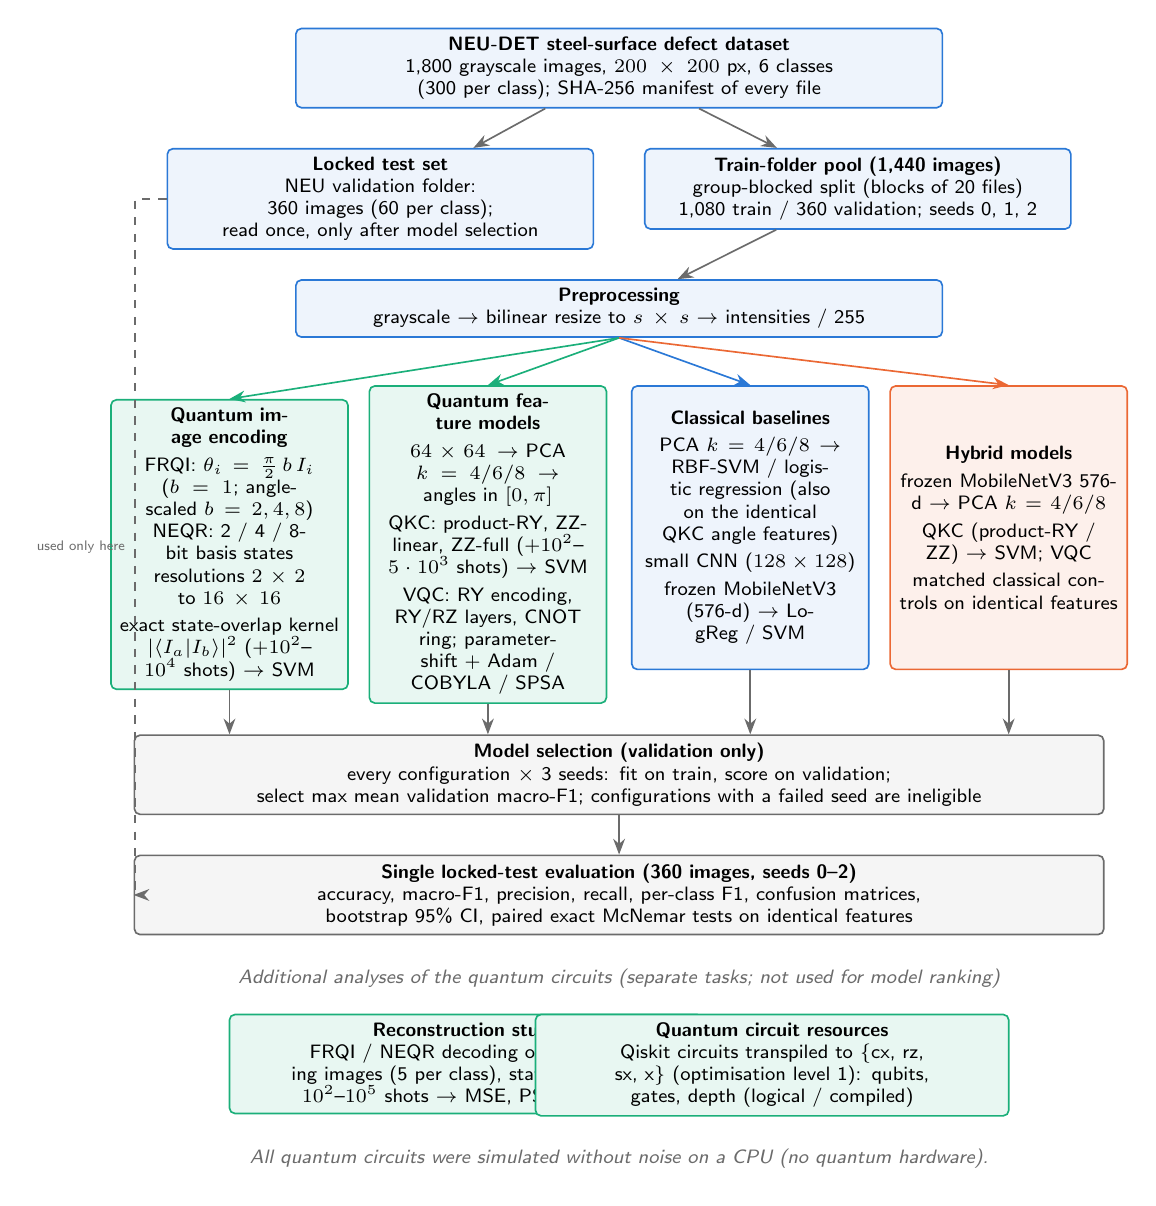
\begin{tikzpicture}[
  font=\sffamily\scriptsize, node distance=4mm and 2.5mm, >={Stealth[length=2mm]},
  base/.style={draw, rounded corners=2pt, line width=0.6pt, align=center, inner sep=3pt},
  data/.style={base, draw=cBlue, fill=cBlue!8, text width=#1},
  quant/.style={base, draw=cAqua, fill=cAqua!10, text width=#1, minimum height=36mm},
  clas/.style={base, draw=cBlue, fill=cBlue!8, text width=#1, minimum height=36mm},
  hyb/.style={base, draw=cOrange, fill=cOrange!10, text width=#1, minimum height=36mm},
  evalb/.style={base, draw=cGrey, fill=black!4, text width=#1},
  qnote/.style={base, draw=cAqua, fill=cAqua!10, text width=#1},
  arr/.style={->, draw=cGrey, line width=0.6pt}]

\node[data=80mm] (ds) {\textbf{NEU-DET steel-surface defect dataset}\\
  1,800 grayscale images, $200\times200$ px, 6 classes (300 per class); SHA-256 manifest of every file};
\node[data=52mm, below left=5mm and -38mm of ds] (test) {\textbf{Locked test set}\\
  NEU validation folder: 360 images (60 per class);\\ read once, only after model selection};
\node[data=52mm, below right=5mm and -38mm of ds] (pool) {\textbf{Train-folder pool (1,440 images)}\\
  group-blocked split (blocks of 20 files)\\ 1,080 train / 360 validation; seeds 0, 1, 2};
\node[data=80mm, below=5mm of $(test.south)!0.5!(pool.south)$] (pre) {\textbf{Preprocessing}\\
  grayscale $\rightarrow$ bilinear resize to $s\times s$ $\rightarrow$ intensities / 255};

\node[quant=28mm, below left=6mm and 1.5mm of pre.south] (q2) {\textbf{Quantum feature models}\\[2pt]
  $64\times64\rightarrow$ PCA $k=4/6/8\rightarrow$ angles in $[0,\pi]$\\[2pt]
  QKC: product-RY, ZZ-linear, ZZ-full (+$10^2$--$5\cdot10^3$ shots) $\rightarrow$ SVM\\[2pt]
  VQC: RY encoding, RY/RZ layers, CNOT ring; parameter-shift + Adam / COBYLA / SPSA};
\node[quant=28mm, left=2.5mm of q2] (q1) {\textbf{Quantum image encoding}\\[2pt]
  FRQI: $\theta_i=\tfrac{\pi}{2}\,b\,I_i$ ($b=1$; angle-scaled $b=2,4,8$)\\
  NEQR: 2 / 4 / 8-bit basis states\\ resolutions $2\times2$ to $16\times16$\\[2pt]
  exact state-overlap kernel $|\langle I_a|I_b\rangle|^2$ (+$10^2$--$10^4$ shots) $\rightarrow$ SVM};
\node[clas=28mm, below right=6mm and 1.5mm of pre.south] (c1) {\textbf{Classical baselines}\\[2pt]
  PCA $k=4/6/8\rightarrow$ RBF-SVM / logistic regression (also on the identical QKC angle features)\\[2pt]
  small CNN ($128\times128$)\\[2pt] frozen MobileNetV3 (576-d) $\rightarrow$ LogReg / SVM};
\node[hyb=28mm, right=2.5mm of c1] (h1) {\textbf{Hybrid models}\\[2pt]
  frozen MobileNetV3 576-d $\rightarrow$ PCA $k=4/6/8$\\[2pt]
  QKC (product-RY / ZZ) $\rightarrow$ SVM; VQC\\[2pt]
  matched classical controls on identical features};

\node[evalb=121mm, below=6mm of $(q2.south)!0.5!(c1.south)$] (sel) {\textbf{Model selection (validation only)}\\
  every configuration $\times$ 3 seeds: fit on train, score on validation;\\
  select max mean validation macro-F1; configurations with a failed seed are ineligible};
\node[evalb=121mm, below=5mm of sel] (fin) {\textbf{Single locked-test evaluation (360 images, seeds 0--2)}\\
  accuracy, macro-F1, precision, recall, per-class F1, confusion matrices,\\
  bootstrap 95\% CI, paired exact McNemar tests on identical features};
\node[below=3mm of fin, font=\sffamily\scriptsize\itshape, text=cGrey] (lab)
  {Additional analyses of the quantum circuits (separate tasks; not used for model ranking)};
\node[qnote=58mm, below=2mm of lab.south west, anchor=north west] (rec) {\textbf{Reconstruction study}\\
  FRQI / NEQR decoding of 30 training images (5 per class), statevector and $10^2$--$10^5$ shots $\rightarrow$ MSE, PSNR, SSIM};
\node[qnote=58mm, below=2mm of lab.south east, anchor=north east] (res) {\textbf{Quantum circuit resources}\\
  Qiskit circuits transpiled to \{cx, rz, sx, x\} (optimisation level 1): qubits, gates, depth (logical / compiled)};
\node[below=3mm of $(rec.south)!0.5!(res.south)$, font=\sffamily\scriptsize\itshape, text=cGrey]
  {All quantum circuits were simulated without noise on a CPU (no quantum hardware).};

\draw[arr] (ds) -- (test);
\draw[arr] (ds) -- (pool);
\draw[arr] (pool) -- (pre);
\foreach \n/\c in {q1/cAqua, q2/cAqua, c1/cBlue, h1/cOrange} {
  \draw[->, draw=\c, line width=0.6pt] (pre.south) -- (\n.north);
  \draw[arr] (\n.south) -- (\n.south |- sel.north);
}
\draw[arr] (sel) -- (fin);
\draw[arr, dashed] (test.west) -- ++(-4mm,0) |- node[pos=0.25, left, font=\sffamily\tiny, text=cGrey] {used only here} (fin.west);
\end{tikzpicture}
\end{document}
